
\chapter{CONCEITOS TEÓRICOS E FUNDAMENTAÇÃO}

Este capítulo tem por objetivo apresentar os conceitos fundamentais que embasam a pesquisa, com ênfase nas áreas de aprendizado profundo, modelos de linguagem natural e sistemas multiagentes aplicados ao diagnóstico automatizado. Cada seção a seguir introduz os principais elementos técnicos e teóricos que sustentam o desenvolvimento do sistema proposto.

\section{Câncer de Pele}
\subsection{Epidemiologia e relevância clínica}

O câncer de pele figura entre as neoplasias mais comuns no mundo, apresentando crescimento contínuo de incidência nas últimas décadas. De acordo com a Agência Internacional para Pesquisa em Câncer (IARC), vinculada à Organização Mundial da Saúde (OMS), estima-se que, em 2022, tenham ocorrido aproximadamente 330 mil novos casos de melanoma e cerca de 60 mil mortes relacionadas à doença \cite{iarc2022skincancer}. Os cânceres de pele não melanoma, por sua vez, são ainda mais prevalentes: segundo o relatório \textit{GLOBOCAN 2022}, cerca de 1,23 milhão de pessoas foram diagnosticadas nesse mesmo período \cite{wang2025global}. Análises recentes do \textit{Global Burden of Disease} indicam que, em 2021, a carga combinada de melanoma e não melanoma atingiu 6,64 milhões de casos em todo o mundo, com taxa de incidência padronizada de 77,66 por 100 mil habitantes \cite{zhou2025global}.

A distribuição geográfica desses casos apresenta forte variação entre regiões, conforme ilustrado na Figura~\ref{fig:epidemiologia}. Observa-se maior risco cumulativo em países de alta latitude e população predominantemente de pele clara, como Austrália, Nova Zelândia, Canadá e nações do norte da Europa, onde a exposição à radiação ultravioleta (UV) é intensa e contínua. Em contrapartida, regiões equatoriais e africanas registram menor incidência, devido à maior pigmentação cutânea e hábitos de fotoproteção natural. Esses dados reforçam o papel dos fatores ambientais e genéticos na etiologia do câncer de pele e evidenciam desigualdades globais na exposição solar e no acesso a medidas preventivas \cite{iarc2022globocan}.

\begin{figure}[H]
	\centering
	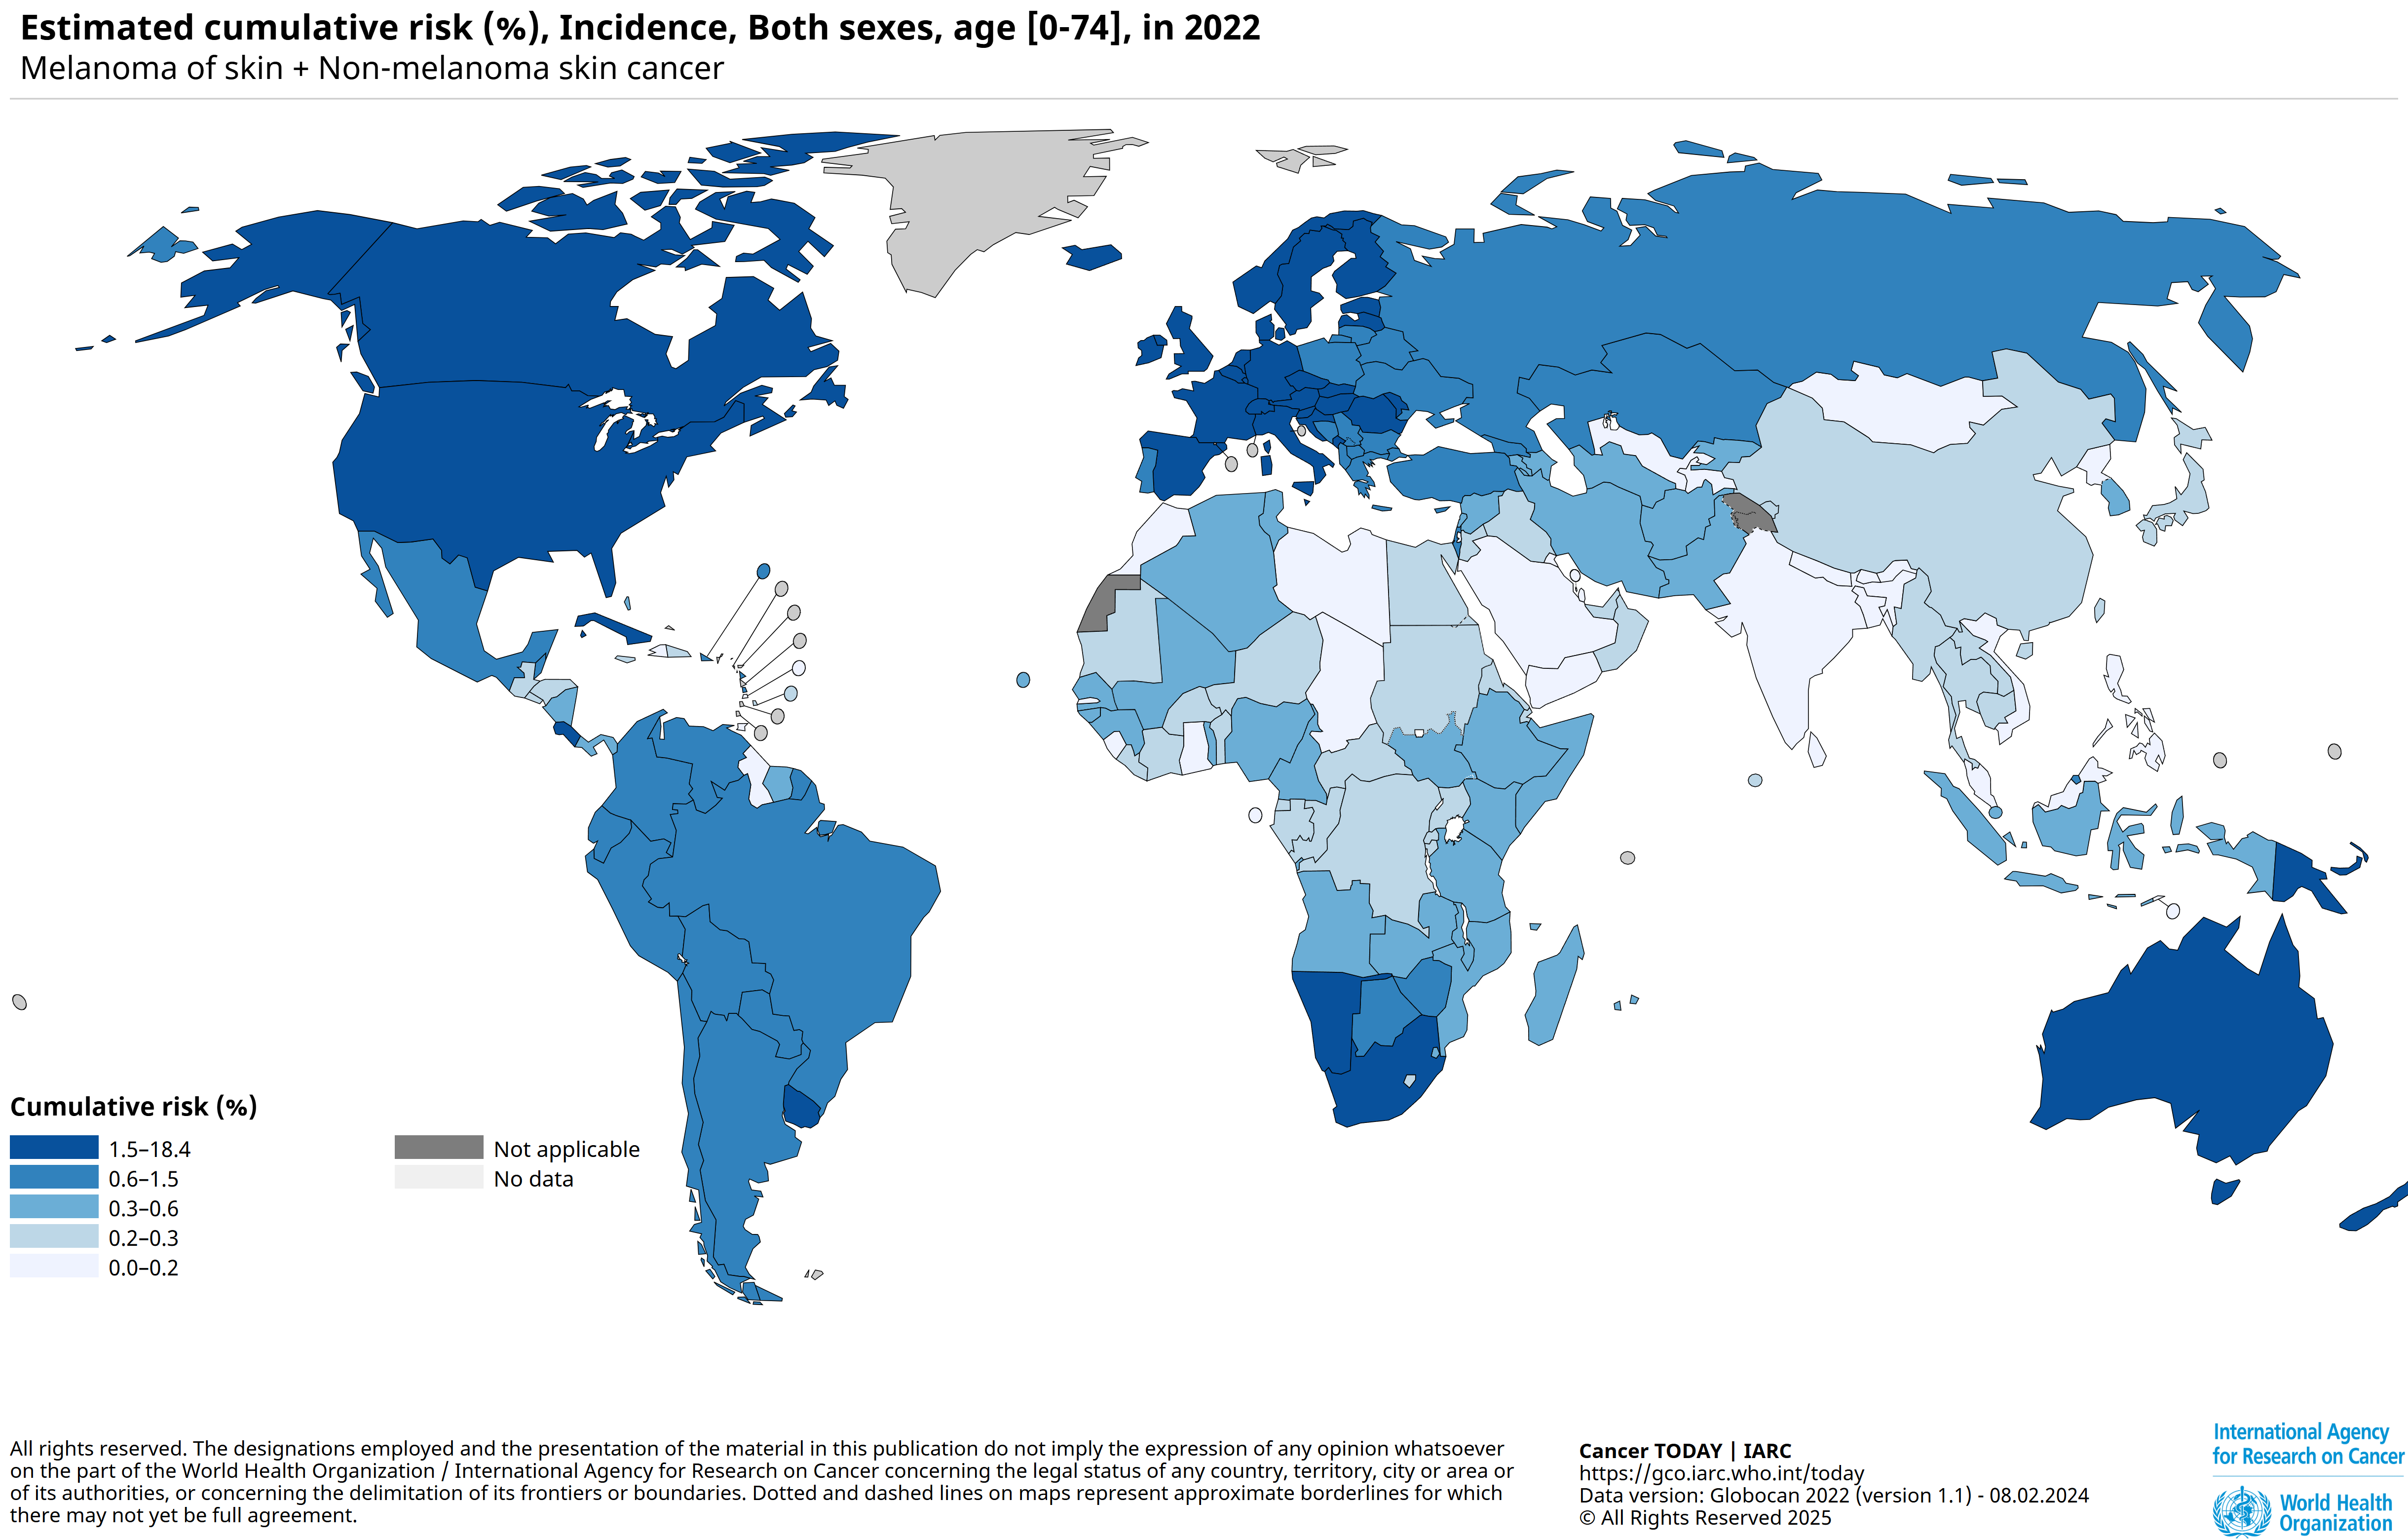
\includegraphics[width=0.95\textwidth]{imagens/Ch2/Sec1.1.png}
	\caption{Risco cumulativo estimado (\%) de incidência de câncer de pele (melanoma e não melanoma), ambos os sexos, entre 0 e 74 anos, em 2022. As áreas em azul-escuro indicam maior risco de desenvolvimento da doença. Fonte: \citeonline{iarc2022globocan}.}
	\label{fig:epidemiologia}
\end{figure}

No Brasil, o câncer de pele representa o tipo mais incidente. O Instituto Nacional de Câncer (INCA) estima que, no triênio 2023–2025, ocorram mais de 220 mil novos casos anuais de câncer de pele não melanoma, correspondendo a aproximadamente 31\% de todos os diagnósticos de câncer no país \cite{inca2023estimativa}. Embora menos frequente, o melanoma é responsável pela maioria das mortes relacionadas ao câncer de pele, devido ao seu alto potencial metastático e rápida progressão em estágios avançados.

A relevância clínica do tema reside na importância do diagnóstico precoce. Estudos epidemiológicos indicam que a taxa de sobrevida em cinco anos para pacientes com melanoma detectado precocemente pode ultrapassar 90\%, enquanto em estágios avançados esse índice pode cair para menos de 20\% \cite{garbe2009melanoma}. Nesse contexto, estratégias de rastreamento e tecnologias de apoio, como sistemas automatizados baseados em inteligência artificial, tornam-se essenciais para ampliar o acesso ao diagnóstico e reduzir a mortalidade em regiões com escassez de especialistas.


\subsection{Características clínicas e dermatoscópicas}

A avaliação clínica inicial das lesões cutâneas suspeitas de melanoma baseia-se amplamente no mnemônico \textit{ABCDE} (\textit{Asymmetry, Border irregularity, Color variegation, Diameter, Evolution}), um método difundido em triagem e educação em saúde. Em termos práticos, lesões assimétricas, com bordas irregulares, variação de cores e diâmetro superior a 6\,mm, ou que apresentem evolução morfológica e cromática recente, devem ser investigadas de forma mais aprofundada \cite{abbasi2004early}. A Figura~\ref{fig:abcd_comparison} ilustra exemplos clínicos de lesões benignas e malignas, evidenciando as diferenças morfológicas e cromáticas associadas a cada condição.

\begin{figure}[H]
	\centering
	\begin{subfigure}[b]{0.45\textwidth}
		\centering
		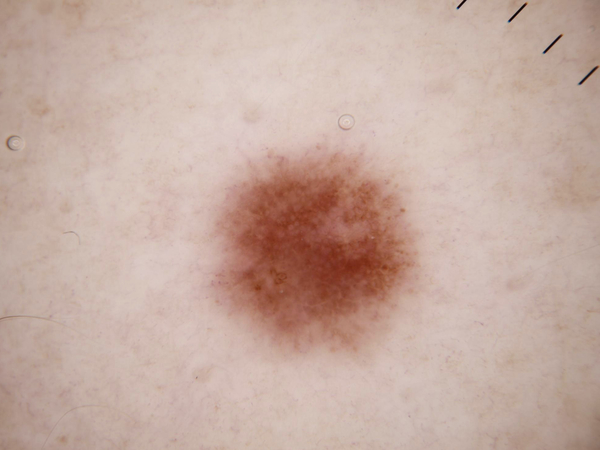
\includegraphics[width=\textwidth]{imagens/Ch2/Sec1.2_Benigna.jpg}
		\caption{Lesão benigna – coloração homogênea e contorno regular.}
		\label{fig:benign_lesion}
	\end{subfigure}
	\hfill
	\begin{subfigure}[b]{0.45\textwidth}
		\centering
		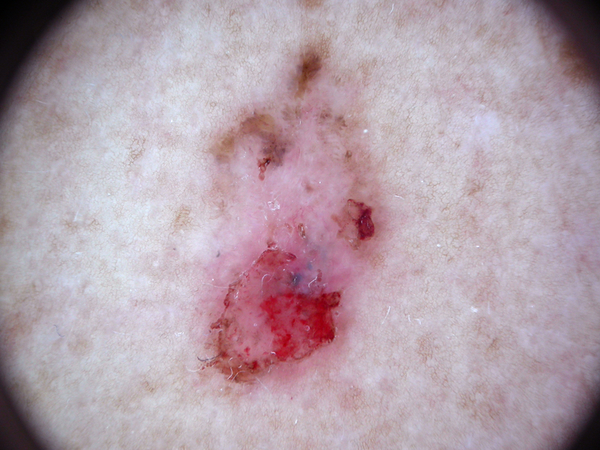
\includegraphics[width=\textwidth]{imagens/Ch2/Sec1.2_Maligna.jpg}
		\caption{Lesão maligna – assimetria, múltiplas cores e bordas irregulares.}
		\label{fig:malignant_lesion}
	\end{subfigure}
	\caption{Comparação visual entre lesões benignas e malignas segundo o método \textit{ABCDE}. A análise clínica considera assimetria, irregularidade de bordas, variação de cor, diâmetro e evolução temporal. Imagens adaptadas do conjunto público ISIC Archive \cite{tschandl2018ham10000}.}
	\label{fig:abcd_comparison}
\end{figure}

Embora simples e de fácil adoção, o \textit{ABCDE} é um instrumento essencialmente clínico-visual, sensível a variações de iluminação, distância focal e resolução da imagem, o que reforça a necessidade de padronização do registro fotográfico, sobretudo em aplicações automatizadas. Em nível submacroscópico, a dermatoscopia adiciona informações estruturais e cromáticas não acessíveis ao exame clínico convencional, aumentando significativamente a acurácia diagnóstica frente à inspeção a olho nu \cite{kittler2002diagnostic}.

Entre os principais algoritmos dermatoscópicos destacam-se: (i) a regra \textit{ABCD da dermatoscopia}, que quantifica Assimetria, Bordas, Cor e Estruturas (\textit{Dermoscopic structures}) mediante pontuação contínua; (ii) o \textit{Seven-Point Checklist} (SPCL), que organiza critérios maiores e menores para indicar probabilidade de melanoma; e (iii) o Método de Menzies, que utiliza dois critérios negativos (padrão simétrico e cor única) e um conjunto de critérios positivos, como véu azul-branco, múltiplos pontos marrons, pseudópodes, \textit{radial streaming}, despigmentação em cicatriz, pontos/glóbulos pretos periféricos e presença de cinco a seis cores \cite{nachbar1994abcd,argenziano2003consensus,argenziano2010sevenpoint,menzies1996frequency}. 

É importante salientar que muitos desses critérios (por exemplo, véu azul-branco, rede pigmentada e pseudópodes) são típicos da dermatoscopia (polarizada ou não) e podem não ser captáveis em fotografias clínicas comuns. Essa distinção é essencial no desenho metodológico: \textit{pipelines} que operam apenas com imagens clínicas devem privilegiar atributos morfológicos globais (assimetria geométrica, irregularidade de contorno, variação global de cor e textura) e medidas derivadas da segmentação (área, razão de eixos, circularidade), reservando a interpretação de estruturas dermatoscópicas para conjuntos de dados adequadamente adquiridos \cite{kittler2002diagnostic,tschandl2018ham10000}. 

De forma convergente, estudos recentes indicam que tanto a análise manual assistida por dermatoscopia quanto modelos computacionais treinados com esse tipo de imagem tendem a superar o desempenho baseado somente em fotografias clínicas, reforçando o ganho de informação desse modo de aquisição \cite{kittler2002diagnostic,haenssle2018man}. No contexto deste trabalho, essa limitação é explicitamente considerada na seleção de características e no desenho dos agentes, de forma a alinhar as expectativas de desempenho às propriedades do dado disponível.


\section{Redes Neurais Artificiais}
\subsection{Fundamentos das RNAs}

\begin{figure}[H]
\centering
\begin{tikzpicture}[
    node distance=12mm,
    every node/.style={circle, draw, minimum size=7mm, inner sep=0pt}
]
% Input layer
\node (x1) at (0,0) {$x_1$};
\node (x2) [below=of x1] {$x_2$};
\node (x3) [below=of x2] {$x_3$};

% Hidden layer
\node (h1) [right=25mm of x1] {$h_1$};
\node (h2) [below=of h1] {$h_2$};
\node (h3) [below=of h2] {$h_3$};

% Output layer
\node (y1) [right=25mm of h2] {$\hat{y}$};

% Connections: input -> hidden
\foreach \i in {x1,x2,x3}
  \foreach \j in {h1,h2,h3}
    \draw[->, line width=0.6pt] (\i) -- (\j);

% Connections: hidden -> output
\foreach \j in {h1,h2,h3}
  \draw[->, line width=0.6pt] (\j) -- (y1);

% Text boxes (optional)
\node[draw=none, align=center] at (0, 1) {Camada\\ de entrada};
\node[draw=none, align=center] at (3.1, 1) {Camada\\ oculta};
\node[draw=none, align=center] at (6.2, 1) {Saída};

\end{tikzpicture}
\caption{Esquema autoral de uma rede neural feedforward (MLP) com uma camada oculta. A figura ilustra a conexão total entre camadas e a noção de transformação não linear.}
\label{fig:mlp_schematic}
\end{figure}


As Redes Neurais Artificiais (RNAs) constituem a base teórica do aprendizado profundo e são inspiradas em mecanismos biológicos do cérebro humano. Seu princípio fundamental consiste em unidades computacionais denominadas neurônios artificiais, organizadas em camadas, que processam sinais de entrada, aplicam funções de ativação e produzem saídas ajustáveis por meio de um processo de treinamento. Esse treinamento é realizado, em geral, pelo algoritmo de retropropagação do erro, que ajusta os pesos das conexões neuronais de forma iterativa até minimizar a função de perda \cite{rumelhart1986learning}.

O avanço das RNAs está intrinsecamente ligado à disponibilidade de dados em larga escala e ao aumento do poder computacional. A partir da década de 2010, o campo de aprendizado profundo (\textit{deep learning}) emergiu como uma abordagem dominante, trazendo inovações arquiteturais que impulsionaram a performance em diversas tarefas, como reconhecimento de imagens, processamento de linguagem natural e diagnóstico médico assistido por computador \cite{lecun2015deep, schmidhuber2015deep}. No contexto da saúde, as RNAs permitem identificar padrões complexos em imagens clínicas que seriam de difícil percepção por métodos convencionais de análise estatística, aumentando a acurácia e reduzindo a variabilidade intra e interobservador.

A relevância das RNAs no diagnóstico médico decorre da sua capacidade de generalização a partir de exemplos rotulados. Ao aprender a mapear representações de alto nível a partir de dados brutos, esses modelos conseguem captar características discriminativas úteis para tarefas como classificação de lesões cutâneas, diferenciação entre imagens normais e patológicas e detecção precoce de anomalias \cite{goodfellow2016deep}. No entanto, o desempenho das RNAs depende fortemente da qualidade dos dados disponíveis, sendo suscetíveis a sobreajuste (\textit{overfitting}) em bases pequenas ou desbalanceadas, o que torna essencial o uso de técnicas complementares, como regularização e aumento de dados (\textit{data augmentation}).


\subsection{Redes Neurais Convolucionais (CNNs)}

As Redes Neurais Convolucionais (CNNs) representam uma evolução das Redes Neurais Artificiais tradicionais, sendo projetadas especificamente para o processamento de dados com estrutura espacial, como imagens bidimensionais. Sua principal inovação reside na aplicação de filtros convolucionais que percorrem a imagem extraindo características locais,  como bordas, texturas e formas,  em diferentes níveis de abstração. Essa estratégia permite reduzir a dimensionalidade dos dados sem perda significativa de informação relevante e explorar de maneira eficiente as correlações espaciais entre pixels \cite{lecun1998gradient}.

A Figura~\ref{fig:lenet_architecture} apresenta a arquitetura clássica da rede LeNet-5, uma das primeiras CNNs bem-sucedidas desenvolvidas por LeCun e colaboradores. O modelo é composto por uma sequência de camadas convolucionais, funções de ativação não lineares, camadas de \textit{subsampling} (ou \textit{pooling}) para redução espacial e camadas totalmente conectadas responsáveis pela classificação final. Essa hierarquia permite que o modelo construa progressivamente representações mais complexas: camadas iniciais detectam padrões simples (como linhas e bordas), enquanto camadas mais profundas aprendem estruturas de maior abstração, como formas e texturas características de lesões cutâneas \cite{krizhevsky2012imagenet}.

\begin{figure}[H]
	\centering
	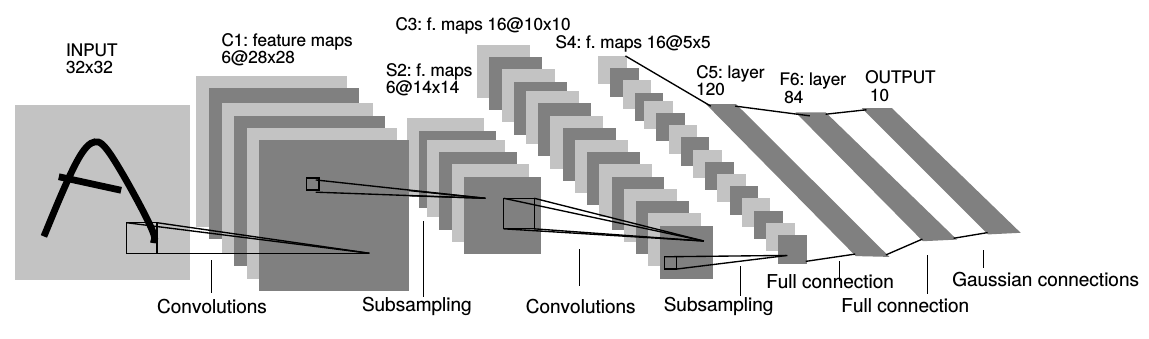
\includegraphics[width=0.95\textwidth]{imagens/Ch2/Sec2.2.png}
	\caption{Arquitetura clássica da rede convolucional LeNet-5, proposta por \citeonline{lecun1998gradient}. A rede é composta por camadas convolucionais intercaladas com operações de \textit{subsampling}, seguidas por camadas totalmente conectadas responsáveis pela classificação. Essa estrutura serviu de base para o desenvolvimento das CNNs modernas.}
	\label{fig:lenet_architecture}
\end{figure}

No campo médico, as CNNs têm demonstrado desempenho superior em tarefas de diagnóstico por imagem, incluindo radiologia, patologia digital e dermatologia. Trabalhos pioneiros mostraram que CNNs podem alcançar resultados comparáveis aos de especialistas humanos na classificação de lesões cutâneas malignas e benignas a partir de imagens dermatoscópicas \cite{esteva2017dermatologist,haenssle2018man}. Essa capacidade decorre da habilidade dessas redes em identificar padrões sutis frequentemente imperceptíveis ao olho humano, fornecendo suporte relevante para decisões clínicas.

Entretanto, a aplicação de CNNs em contextos médicos apresenta desafios particulares. Entre eles estão a necessidade de grandes volumes de dados anotados com precisão, o risco de sobreajuste (\textit{overfitting}) em conjuntos reduzidos e a limitada interpretabilidade dos modelos, frequentemente descritos como “caixas-pretas” \cite{holzinger2017we}. Para mitigar essas limitações, pesquisas recentes têm explorado o uso de arquiteturas híbridas e técnicas de explicabilidade, como \textit{Grad-CAM}, que permitem visualizar as regiões da imagem mais relevantes para a decisão do modelo, aumentando a transparência e a confiança clínica.


\subsection{Redes de Atenção e Transformers}

O mecanismo de atenção foi introduzido como uma solução para superar as limitações dos modelos sequenciais tradicionais, como as redes neurais recorrentes (RNNs), que apresentavam dificuldades em capturar dependências de longo alcance em tarefas de processamento de linguagem natural. A atenção permite que o modelo atribua pesos diferenciados a partes distintas da entrada, concentrando-se seletivamente nas informações mais relevantes para a tarefa em execução \cite{bahdanau2014neural}. 

Esse conceito foi expandido pelo \textit{Transformer}, proposto por \citeonline{vaswani2017attention}, que substituiu completamente a recorrência pelo uso de múltiplos cabeçalhos de atenção (\textit{multi-head attention}) e mecanismos de normalização, tornando-se o paradigma dominante em modelos de linguagem. A Figura~\ref{fig:transformer_architecture} ilustra a arquitetura básica do Transformer, composta por blocos de \textit{encoder} e \textit{decoder}, nos quais o mecanismo de atenção é aplicado em paralelo a camadas de normalização e redes alimentadas adiante (\textit{feed-forward}).

\begin{figure}[H]
	\centering
	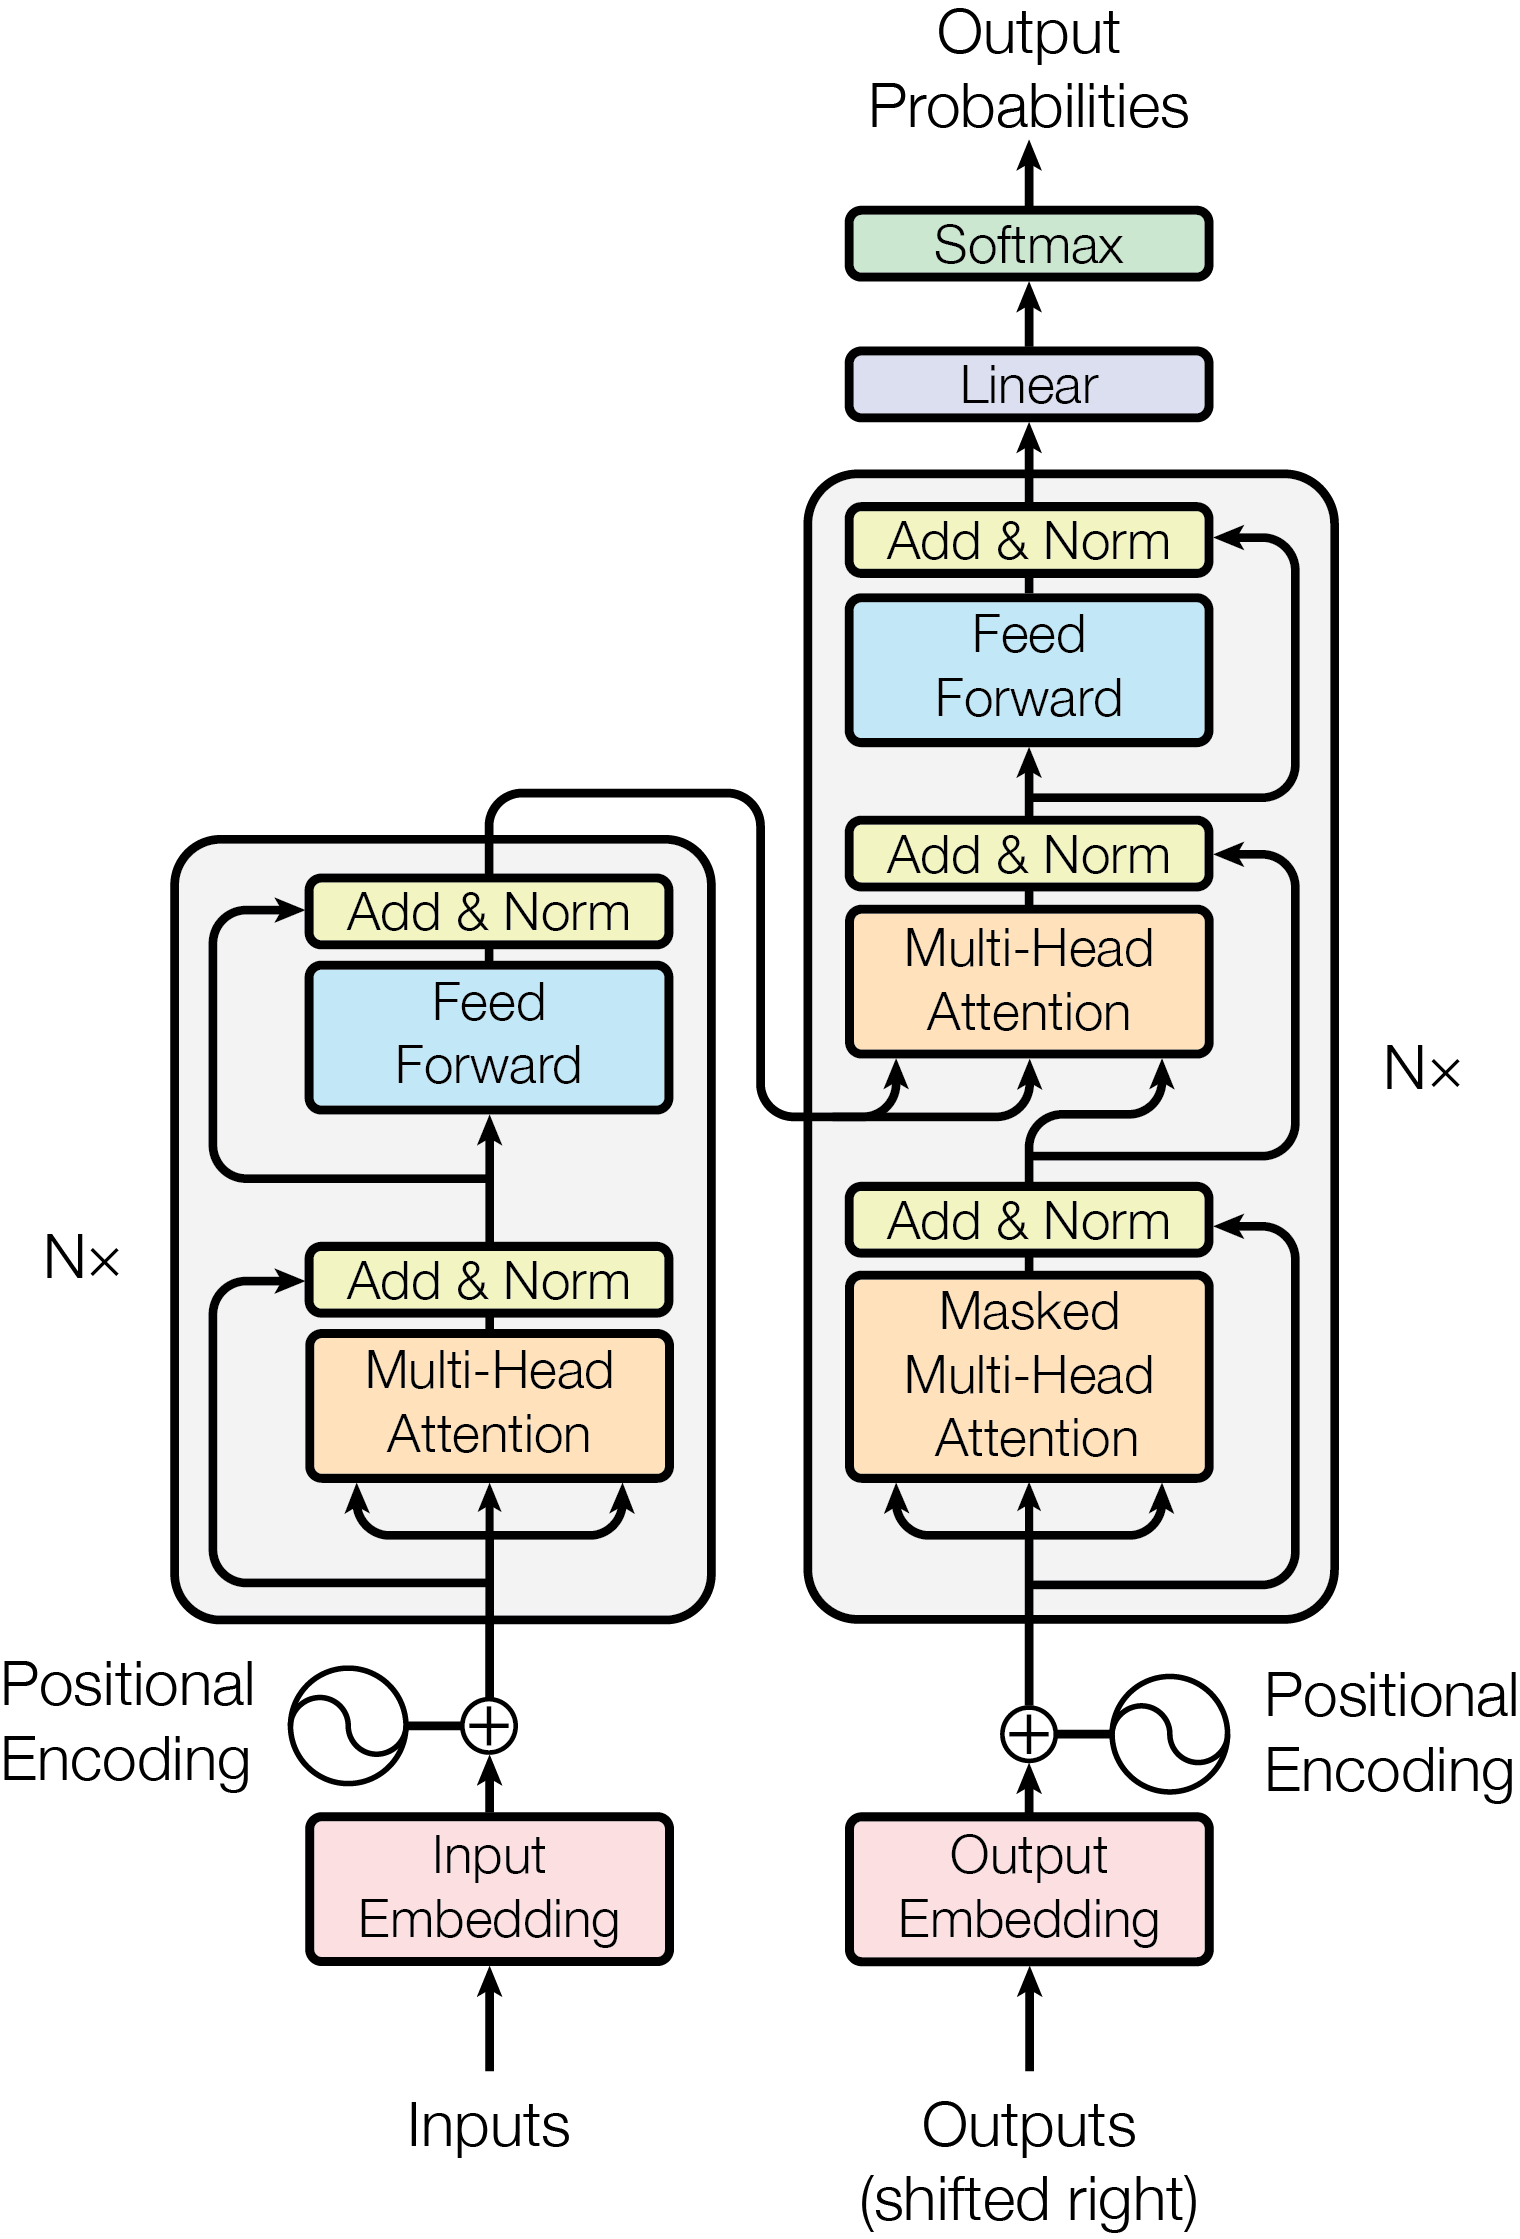
\includegraphics[width=0.85\textwidth]{imagens/Ch2/Sec2.4.png}
	\caption{Arquitetura do modelo Transformer proposto por \citeonline{vaswani2017attention}, composta por blocos de \textit{encoder} e \textit{decoder} conectados por mecanismos de atenção multi-cabeças. Essa estrutura permitiu substituir totalmente a recorrência e impulsionou o desenvolvimento de modelos de linguagem e visão em larga escala.}
	\label{fig:transformer_architecture}
\end{figure}

Nos últimos anos, a arquitetura Transformer ultrapassou o domínio textual e passou a ser aplicada ao processamento de imagens, originando os \textit{Vision Transformers} (ViT). Nessa abordagem, a imagem é dividida em pequenos blocos (\textit{patches}) que são tratados como sequências análogas a palavras em um texto, permitindo ao modelo aprender representações globais da cena \cite{dosovitskiy2021an}. Essa capacidade de modelar relações de longo alcance entre regiões da imagem contrasta com a natureza local das convoluções em CNNs, tornando os Transformers especialmente eficazes em capturar padrões estruturais complexos e contextuais.

No campo da saúde, os Transformers têm se mostrado competitivos ou mesmo superiores às CNNs em diversas tarefas, incluindo classificação de radiografias, análise histopatológica e segmentação de lesões cutâneas. Arquiteturas híbridas, como a TransUNet, combinam convoluções nas etapas iniciais para extrair detalhes locais e módulos de atenção para capturar dependências globais, atingindo resultados de ponta em segmentação médica \cite{chen2021transunet}. Em dermatologia, estudos recentes demonstram que modelos baseados em Transformers podem superar CNNs tradicionais na classificação de imagens de melanoma e outras lesões pigmentadas, especialmente quando aliados a abordagens multimodais que integram dados clínicos e visuais \cite{liu2021swin,raghu2021vision}.

Apesar dos avanços, desafios persistem quanto ao alto custo computacional do treinamento de Transformers e à necessidade de grandes volumes de dados anotados para evitar sobreajuste. Em contextos médicos, nos quais os conjuntos de dados são frequentemente limitados, estratégias como \textit{transfer learning}, autoaprendizado e pré-treinamento multimodal têm se mostrado essenciais para viabilizar sua aplicação prática \cite{khan2022transformers}.


\section{Segmentação de Imagens}
\label{sec:segmentacao}

A segmentação de imagens médicas representa uma das etapas mais fundamentais do processamento computacional em saúde, pois possibilita a identificação precisa de estruturas anatômicas e patológicas, permitindo a quantificação de áreas de interesse e a extração de descritores morfológicos relevantes. Essa técnica é empregada de forma transversal em diversas modalidades diagnósticas, desde exames de imagem de alta resolução até registros clínicos convencionais. A Figura~\ref{fig:segmentacao_medica_exemplos} ilustra esse caráter generalista, apresentando exemplos de segmentação em ressonância magnética cerebral, dermatoscopia e tomografia computadorizada pulmonar.

As três modalidades representadas não têm o objetivo de comparação direta, mas de evidenciar a natureza universal do processo de segmentação,  um mesmo princípio algorítmico capaz de isolar regiões de interesse sob diferentes perspectivas e condições de aquisição. Em ressonância magnética, a segmentação permite delimitar tumores cerebrais e quantificar volumes afetados, contribuindo para protocolos de neurocirurgia e acompanhamento terapêutico \cite{minaee2021image}. Em dermatoscopia, a técnica destaca as fronteiras entre a lesão pigmentada e a pele saudável, fornecendo uma base morfológica para classificadores que diferenciam lesões benignas e malignas \cite{tschandl2018ham10000}. Já em tomografia computadorizada, é aplicada na detecção e mensuração de nódulos pulmonares, oferecendo suporte ao rastreamento precoce de neoplasias \cite{shen2017deep}.

A escolha dessas representações se justifica pela coerência conceitual entre os domínios: embora as propriedades ópticas, os artefatos e os parâmetros físicos variem entre modalidades, o núcleo computacional da segmentação,  baseado em extração hierárquica de características espaciais e reconstrução morfológica,  permanece o mesmo. Essa convergência técnica reforça a plausibilidade de estender arquiteturas já consolidadas, como a U-Net \cite{ronneberger2015unet}, ao domínio da dermatologia. No contexto desta pesquisa, a segmentação é concebida não apenas como um pré-processamento visual, mas como a etapa estruturante que possibilita a análise textual posterior por modelos de linguagem natural e agentes colaborativos, sustentando assim a integração entre visão computacional e raciocínio clínico automatizado.

\begin{figure}[H]
	\centering
	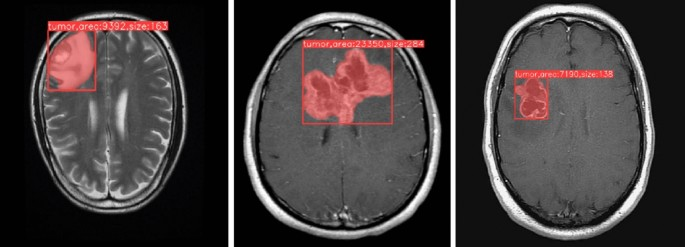
\includegraphics[width=0.32\textwidth]{imagens/Ch2/Sec2.3.Intro1.jpg}
	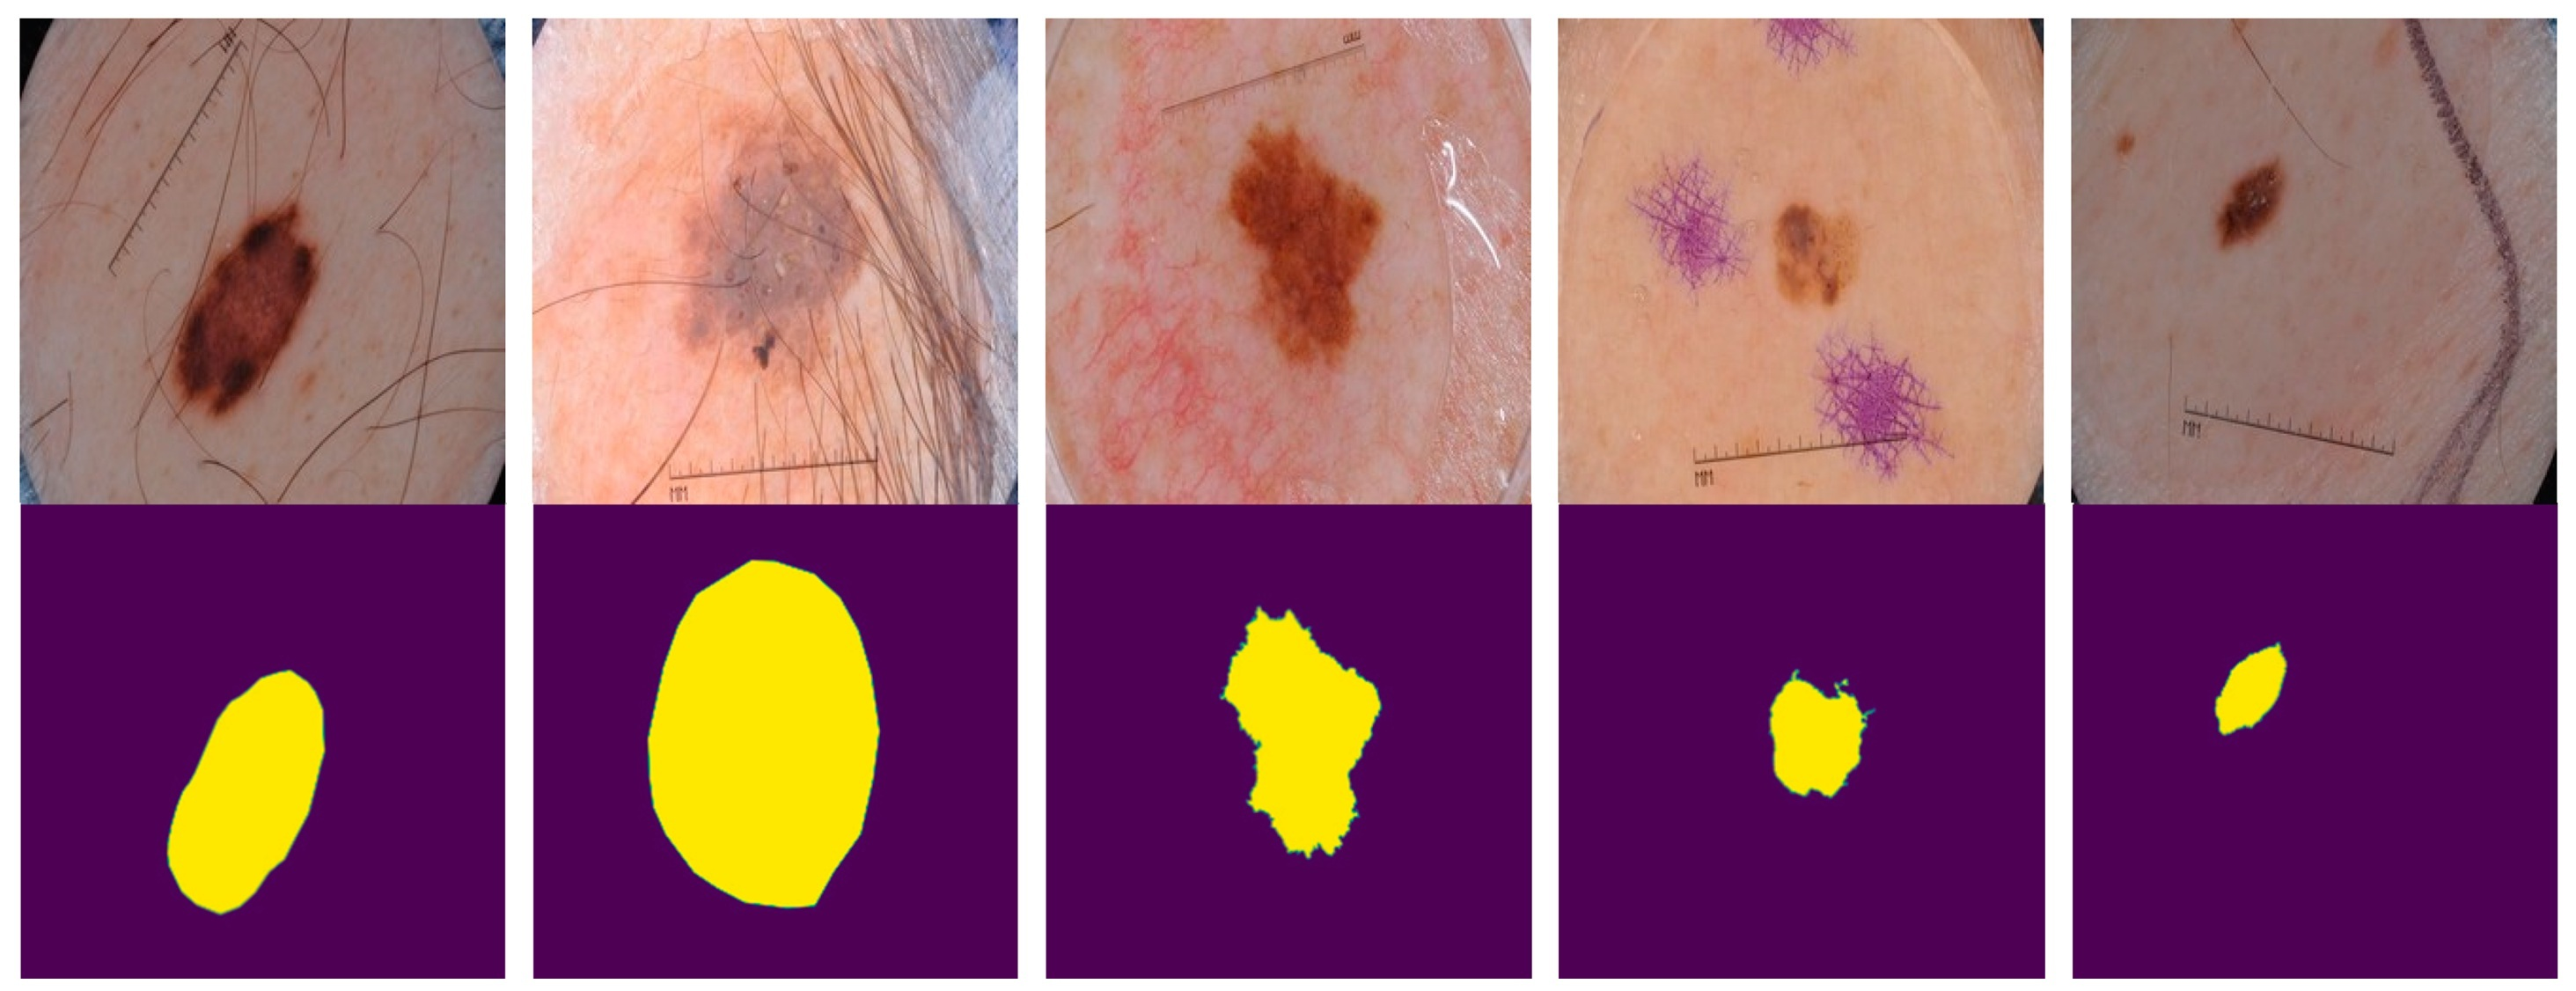
\includegraphics[width=0.32\textwidth]{imagens/Ch2/Sec2.3.Intro2.jpg}
	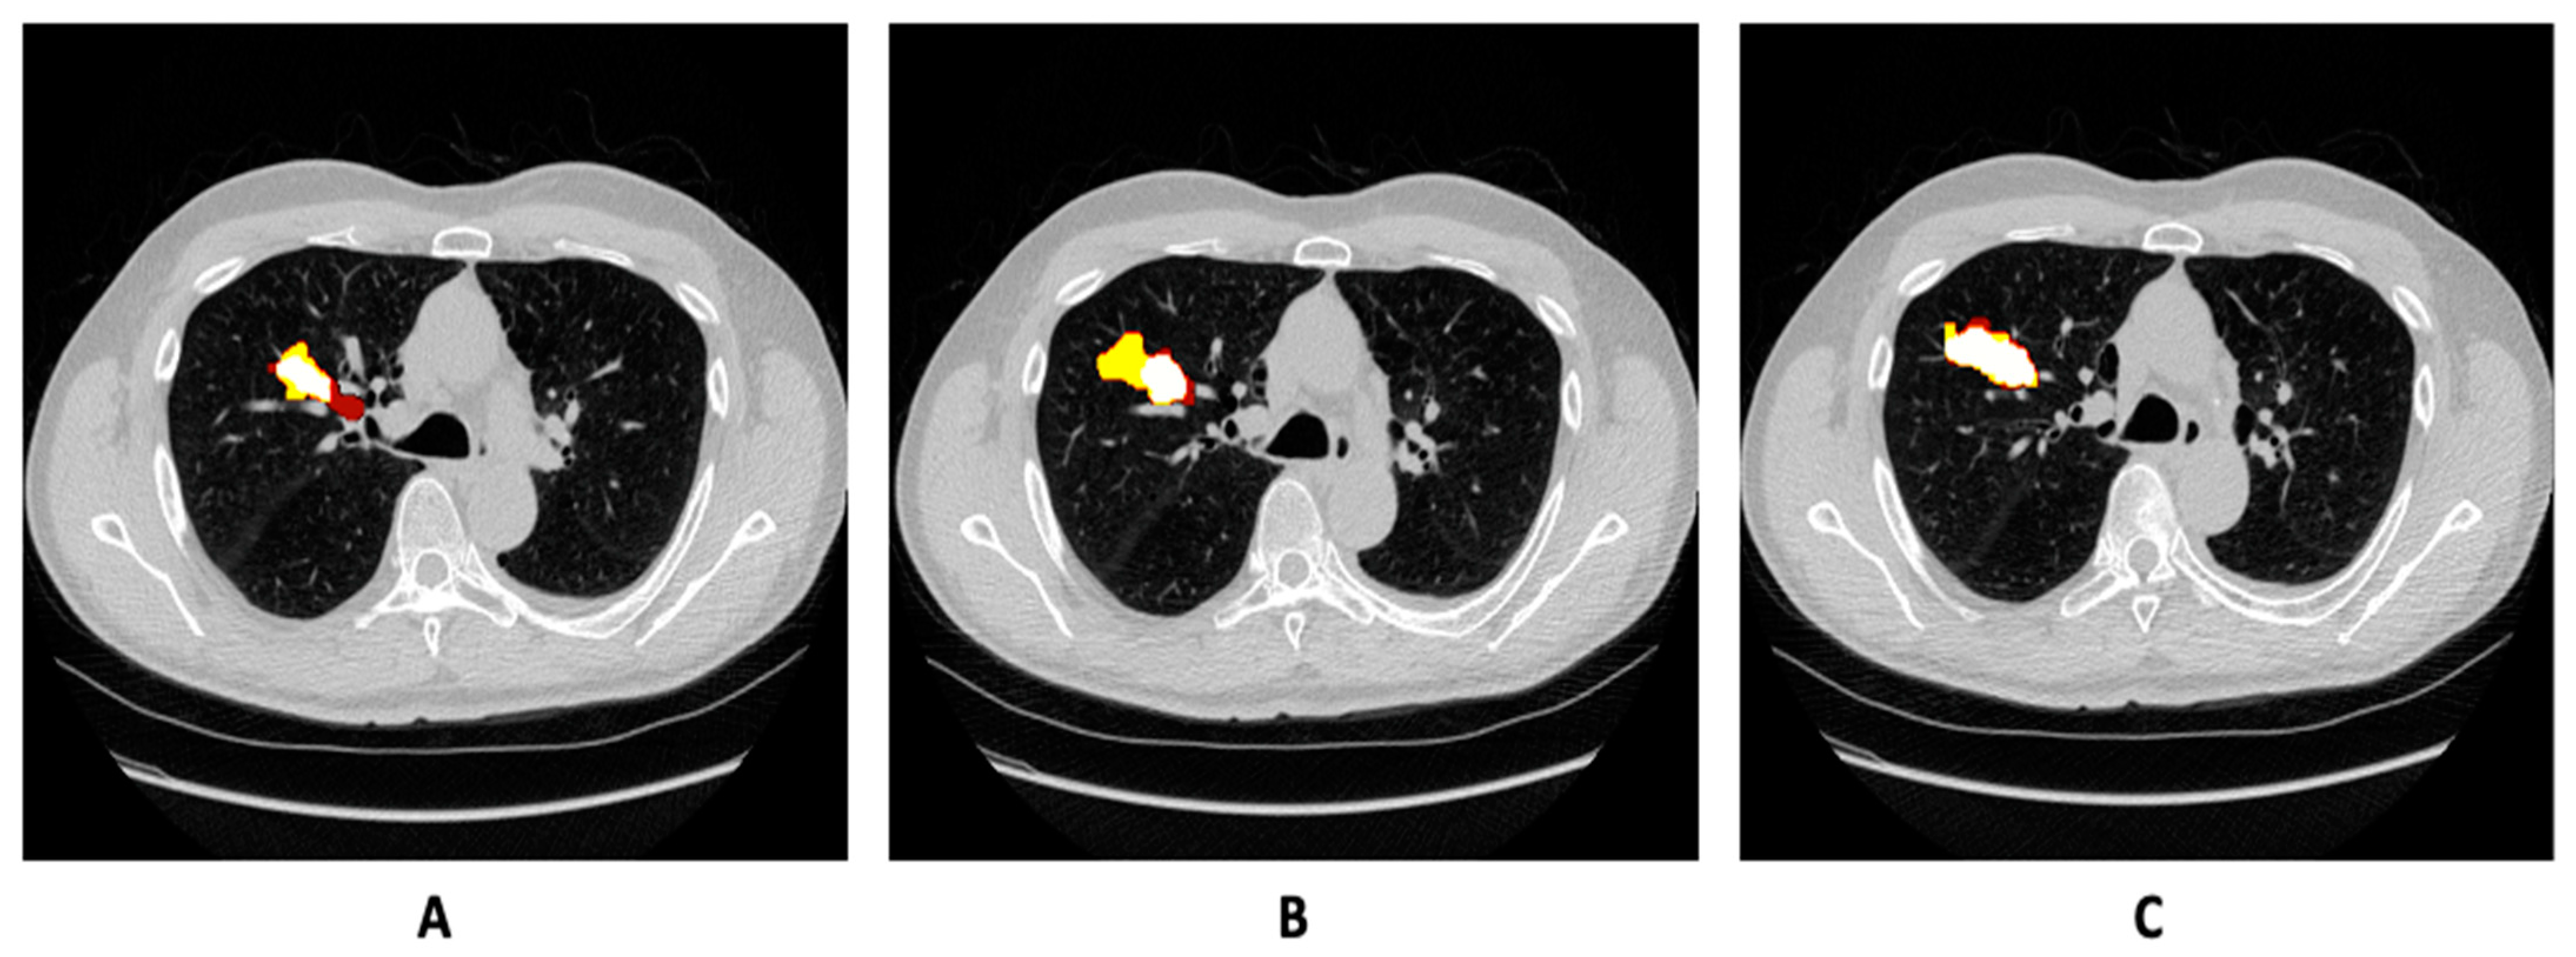
\includegraphics[width=0.32\textwidth]{imagens/Ch2/Sec2.3.Intro3.jpg}
	\caption{
		Exemplos de aplicação da segmentação em diferentes modalidades médicas: 
		(A) delineamento de tumor cerebral em ressonância magnética \cite{minaee2021image}, 
		(B) isolamento de lesão cutânea pigmentada em dermatoscopia \cite{tschandl2018ham10000}, e 
		(C) segmentação de nódulos pulmonares em tomografia computadorizada \cite{shen2017deep}.
		As imagens foram reproduzidas e adaptadas de seus respectivos estudos para fins ilustrativos e acadêmicos.}
	\label{fig:segmentacao_medica_exemplos}
\end{figure}

\subsection{Tipos de Segmentação de Imagens Médicas}

A segmentação de imagens médicas constitui uma das tarefas mais fundamentais em visão computacional aplicada à saúde, permitindo a delimitação precisa de regiões anatômicas ou patológicas de interesse. Diferentes abordagens de segmentação variam quanto ao nível de granularidade e ao tipo de inferência produzida, influenciando diretamente a interpretabilidade e a aplicabilidade clínica do resultado \cite{reinke2021commonlimitations}.

A Figura~\ref{fig:segmentacao_tipos} ilustra, de forma esquemática, os quatro principais paradigmas de predição em visão computacional médica:  
(A) \textbf{classificação de imagem}, na qual a decisão é global e a imagem é associada a um único rótulo;  
(B) \textbf{segmentação semântica}, que rotula cada pixel de acordo com sua classe, permitindo a identificação contínua de regiões homogêneas;  
(C) \textbf{detecção de objetos}, que reconhece e localiza instâncias individuais por meio de \textit{bounding boxes}; e  
(D) \textbf{segmentação por instância}, que combina as abordagens anteriores, distinguindo múltiplos objetos da mesma classe \cite{reinke2021commonlimitations}.

No contexto dermatológico, a \textbf{segmentação semântica} é a mais apropriada, pois as lesões cutâneas tendem a compor uma única estrutura contínua. Nesse caso, o foco analítico recai sobre a geometria da lesão,  área, borda, assimetria e variação de cor,  e não sobre a distinção entre instâncias múltiplas. Essa característica torna o problema mais alinhado a uma formulação pixel a pixel, em que a precisão dos limites é mais relevante do que a diferenciação entre objetos. 

Além disso, o uso da segmentação semântica apresenta vantagens computacionais e metodológicas para integração com sistemas baseados em linguagem natural. Ao delimitar a área de interesse de forma consistente e explicável, o modelo gera uma entrada visual estruturada que pode ser convertida em descrições clínicas compreensíveis por modelos de linguagem (LLMs). Assim, o equilíbrio entre granularidade e interpretabilidade faz da segmentação semântica uma escolha técnica e clinicamente fundamentada para o escopo desta pesquisa.

\begin{figure}[H]
	\centering
	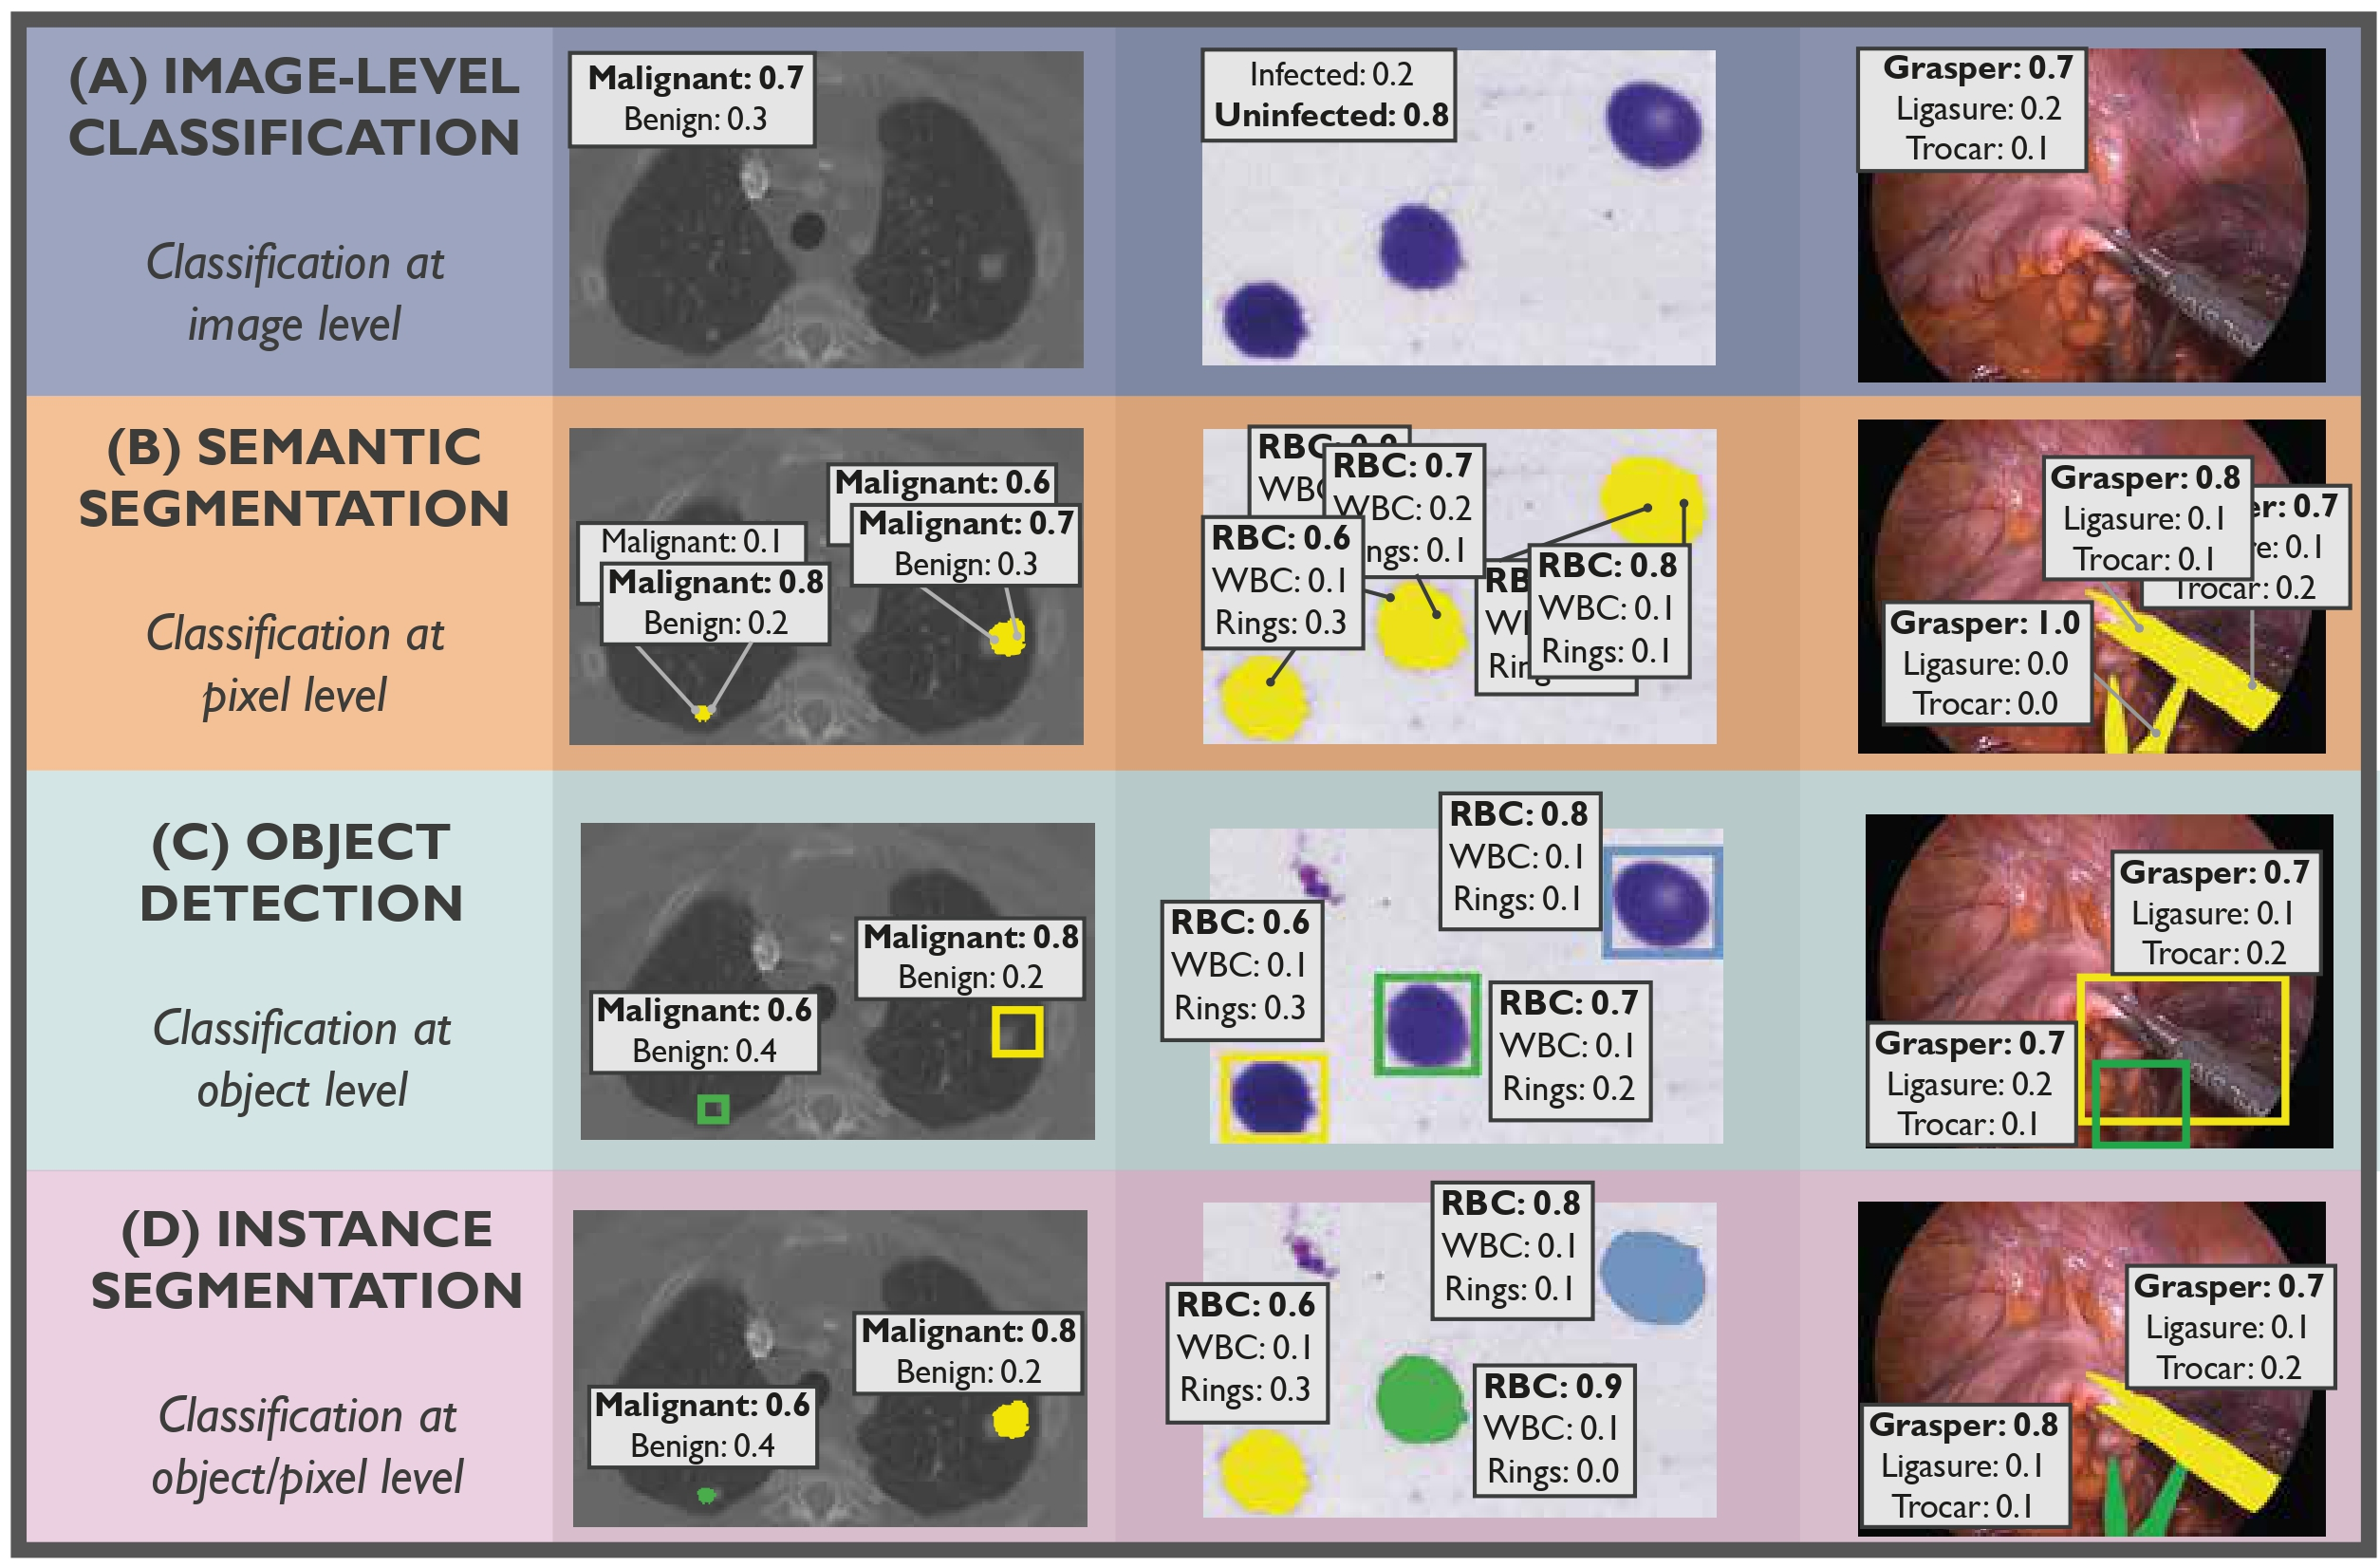
\includegraphics[width=\textwidth]{imagens/Ch2/Section2.3.2.jpg}
	\caption{
		Comparação entre níveis de granularidade em tarefas de visão computacional aplicadas à medicina:
		(A) classificação de imagem,  decisão global por rótulo;
		(B) segmentação semântica,  classificação por pixel;
		(C) detecção de objetos,  reconhecimento e localização de instâncias por caixas delimitadoras; 
		(D) segmentação por instância,  diferenciação individual de múltiplos objetos de mesma classe.
		Adaptado de \citeonline{reinke2021commonlimitations}.}
	\label{fig:segmentacao_tipos}
\end{figure}


\subsection{Arquiteturas baseadas em U-Net}

Desde sua introdução em 2015, a U-Net tornou-se a arquitetura de referência para segmentação de imagens médicas, oferecendo uma combinação eficiente entre simplicidade estrutural e alta capacidade de generalização \cite{ronneberger2015unet}. Sua estrutura em formato de “U”, composta por um caminho de codificação (\textit{encoder}) e outro de decodificação (\textit{decoder}) conectados por \textit{skip connections}, permite extrair características em múltiplas escalas e recuperar informações espaciais perdidas durante o processo de compressão, como ilustrado na Figura~\ref{fig:unet_original}. Essa arquitetura mostrou-se particularmente eficaz em contextos de dados limitados e altamente desbalanceados, como na segmentação de tecidos biológicos, e é apresentada aqui como referência canônica que fundamenta tanto o conceito de \textit{ground truth} de segmentação adotado nesta pesquisa quanto as direções de trabalho futuro.

\begin{figure}[H]
	\centering
	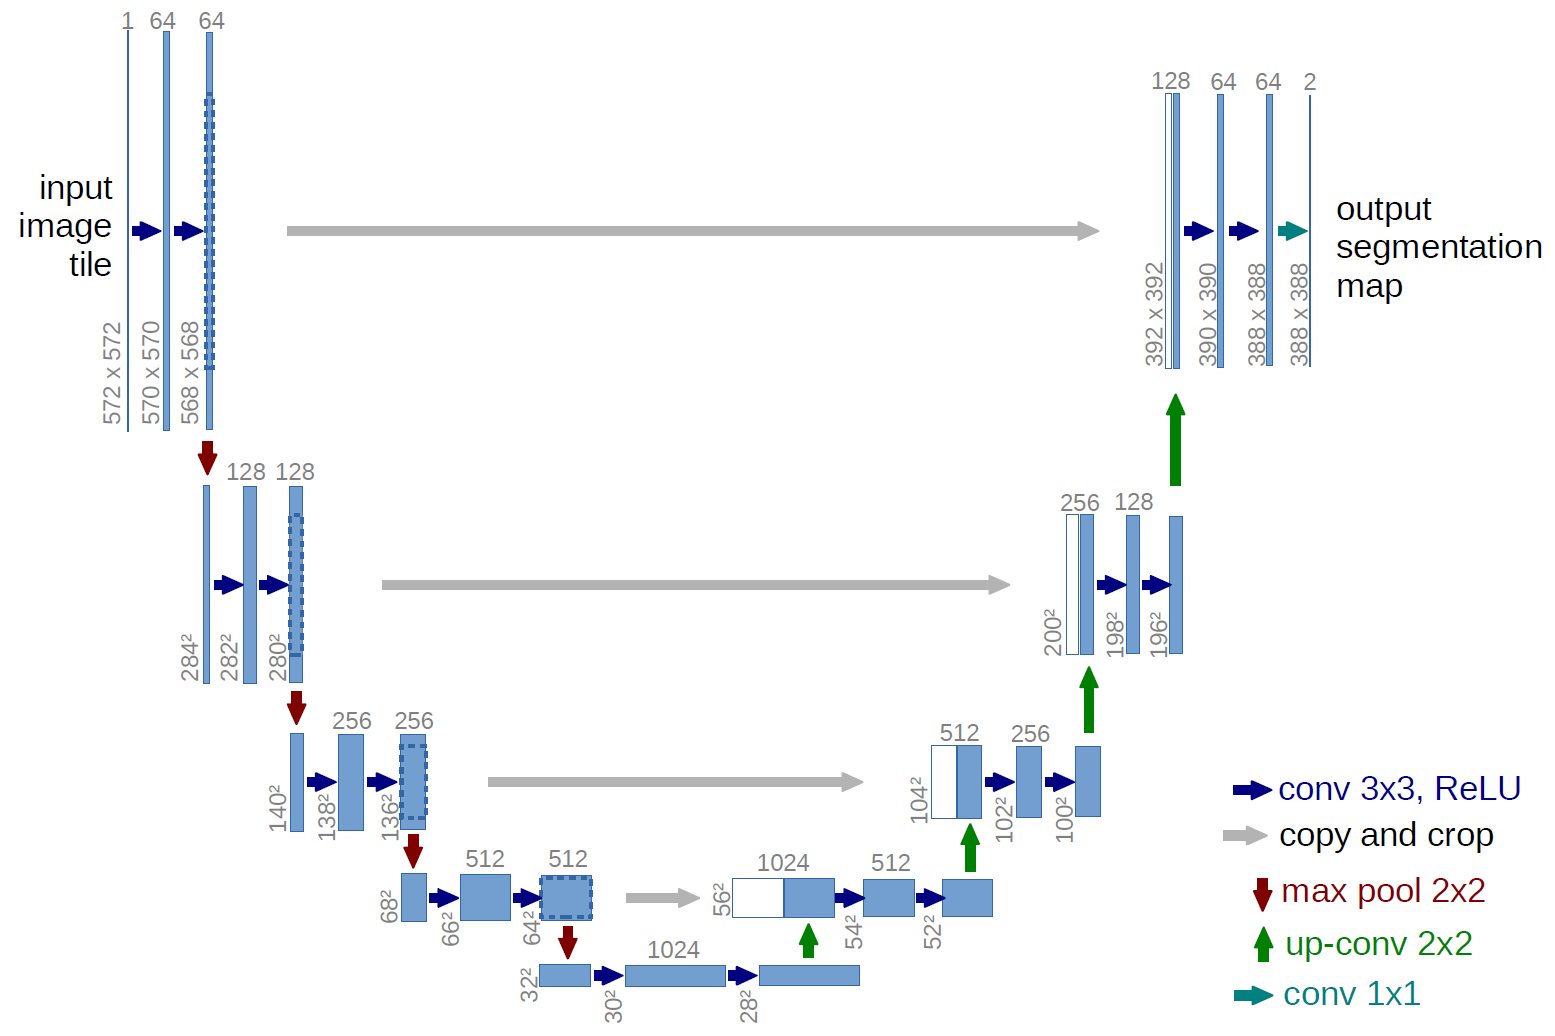
\includegraphics[width=0.9\textwidth]{imagens/Ch2/Sec2.3.png}
	\caption{
		Arquitetura da U-Net clássica \cite{ronneberger2015unet}, composta por um caminho de contração (\textit{encoder}) e um de expansão (\textit{decoder}) conectados por \textit{skip connections}. Essa estrutura permite capturar e reconstruir informações espaciais multiescalares, tornando-a referência em segmentação biomédica.
	}
	\label{fig:unet_original}
\end{figure}

A partir da U-Net clássica, a literatura biomédica desenvolveu variantes que aprimoram aspectos específicos do fluxo de informação. A R2U-Net \cite{alom2018r2unet} incorpora blocos residuais com convoluções recursivas, melhorando a estabilidade de gradiente e a precisão em bordas finas. A Attention U-Net \cite{oktay2018attentionunet} adiciona módulos de atenção espacial nas \textit{skip connections}, permitindo que o modelo suprima automaticamente regiões de fundo e concentre o processamento na lesão, vantagem especialmente relevante em dermatoscopia, onde a lesão ocupa uma fração pequena da cena. A Attention R2U-Net \cite{alom2019attentionr2unet} combina as duas abordagens anteriores, integrando convoluções recursivas e atenção espacial em uma única arquitetura de maior estabilidade e seletividade.

Em síntese, as variantes da U-Net representam uma progressão natural de refinamentos estruturais, que buscam equilibrar desempenho, interpretabilidade e custo computacional. No contexto da presente pesquisa, essas arquiteturas são apresentadas como referencial teórico consolidado para segmentação dermoscópica. A decisão metodológica de adotar as máscaras de referência (\textit{ground truth}) do conjunto PH2 em lugar de segmentações automáticas não invalida sua relevância: ao eliminar a variabilidade introduzida por erros de segmentação, é possível atribuir as diferenças de desempenho exclusivamente à capacidade de raciocínio das LLMs. A integração de um módulo de segmentação automático ao \textit{pipeline} constitui uma direção natural para trabalhos futuros.



\section{Modelos de Linguagem de Larga Escala (LLMs)}

\subsection{Fundamentos}

Os Modelos de Linguagem de Larga Escala (LLMs, do inglês \textit{Large Language Models}) são arquiteturas de aprendizado profundo, em geral baseadas em Transformers, treinadas sobre grandes volumes de dados textuais. Eles possuem bilhões de parâmetros e aprendem representações semânticas que permitem realizar tarefas de compreensão, geração e raciocínio textual \cite{devlin2019bert,brown2020language}. Diferentemente de abordagens anteriores em processamento de linguagem natural (PLN), que eram altamente dependentes de recursos linguísticos manuais, os LLMs capturam padrões complexos diretamente a partir de dados em larga escala, tornando-se modelos de propósito geral capazes de adaptação a múltiplos domínios.

Esses modelos demonstraram desempenho acima do esperado em tarefas de múltipla escolha, resolução de problemas, geração de explicações e sumarização. Sua principal inovação reside na capacidade de generalizar conhecimento aprendido em contextos amplos e aplicá-lo em domínios específicos, frequentemente com pouco ou nenhum ajuste adicional (\textit{zero-shot} e \textit{few-shot learning}) \cite{openai2023gpt4}. No campo da saúde, essa característica é particularmente relevante, visto que permite adaptar o modelo a tarefas médicas sem a necessidade de treinamento extenso em bases clínicas.

\subsection{LLMs com capacidade multimodal}

Uma evolução dos LLMs é a incorporação de entradas multimodais, como imagens e texto. Modelos multimodais, como GPT-5.4-nano \cite{openai2025gpt5nano}, Gemini-3.1-flash-lite \cite{google2025gemini31} e LLaVA \cite{liu2023visual}, são capazes de analisar simultaneamente descrições clínicas e imagens, ampliando sua aplicabilidade em diagnósticos médicos. Essa capacidade torna possível integrar informações visuais (lesões, radiografias, histopatologia) e contextuais (histórico clínico, sintomas relatados), aproximando a inteligência artificial da prática diagnóstica real.

No campo da dermatologia, essa integração já vem sendo explorada em sistemas que combinam imagens de lesões cutâneas e descrições clínicas, permitindo a geração de relatórios estruturados e recomendações diagnósticas. Estudos recentes demonstram que tais modelos podem alcançar acurácia comparável à de especialistas em triagem de melanoma e outras neoplasias cutâneas, além de oferecer explicações em linguagem natural que facilitam a auditabilidade \cite{nori2023capabilitiesgpt4medicalchallenge,vashisht2024umassbionlpmediqam3g2024dermprompt}. 

\subsection{Desafios e limitações em saúde}

Apesar do potencial, a aplicação de LLMs em medicina enfrenta desafios importantes. Um deles é a ocorrência de alucinações, quando o modelo gera informações plausíveis, porém incorretas, que podem comprometer decisões clínicas \cite{rao2023large}. Outro aspecto crítico refere-se à confiabilidade: embora sejam poderosos, os LLMs não foram originalmente projetados para contextos de alto risco como a saúde, exigindo validação rigorosa e supervisão humana constante. Além disso, há questões éticas associadas ao uso de dados sensíveis, como privacidade e viés algorítmico, que podem impactar a equidade no acesso a diagnósticos \cite{tang2023evaluating}.

Essas limitações indicam que os LLMs devem ser considerados ferramentas de apoio, e não substitutos de especialistas. Estratégias como o ajuste fino supervisionado (\textit{fine-tuning}) em bases clínicas, a incorporação de mecanismos de explicabilidade e a integração com sistemas de recuperação de conhecimento (\textit{Retrieval-Augmented Generation}, RAG) são caminhos promissores para aumentar a robustez e a confiabilidade de sua aplicação em saúde.


\section{Sistemas Multiagentes}

\subsection{Fundamentos}

Sistemas Multiagentes (SMAs) são compostos por múltiplas entidades autônomas, denominadas agentes, que interagem em um ambiente compartilhado para resolver problemas complexos de forma cooperativa ou competitiva. Cada agente é caracterizado por sua autonomia, capacidade de percepção do ambiente, habilidade de comunicação e competência para tomar decisões baseadas em objetivos individuais ou coletivos \cite{wooldridge2009introduction}. Diferentemente de sistemas centralizados, os SMAs apresentam maior robustez e escalabilidade, uma vez que o comportamento global emerge da interação distribuída entre agentes especializados, sem a necessidade de um controle único.

A Figura~\ref{fig:multiagent_architecture} ilustra a arquitetura multiagente proposta nesta pesquisa. Nesse fluxo, o processo inicia-se com a entrada das máscaras de segmentação de referência (\textit{ground truth}) do conjunto PH2, que são avaliadas paralelamente por três agentes diagnósticos especializados em protocolos clínicos distintos: o \textit{agente ABCD} (\textit{diagnostic\_abcd}), o \textit{agente Menzies} (\textit{diagnostic\_menzies}) e o \textit{agente SPCL} (\textit{diagnostic\_spcl}, \textit{Seven-Point Checklist}). Cada agente aplica seu protocolo de forma independente, produzindo uma avaliação complementar sobre a mesma lesão. Em seguida, um agente sumarizador (\textit{summary}) consolida as avaliações parciais em um diagnóstico unificado, que é posteriormente revisado criticamente por um agente validador (\textit{critical\_review}). Essa estrutura permite a integração de diferentes perspectivas clínicas e a redução de vieses individuais na inferência final.

\begin{figure}[H]
	\centering
	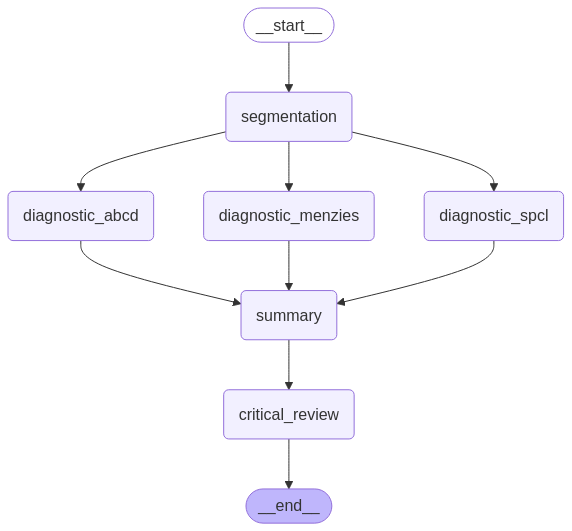
\includegraphics[width=0.8\textwidth]{imagens/Ch2/Sec4.1.png}
	\caption{Arquitetura geral do sistema multiagente desenvolvido. O fluxo inicia com as máscaras de segmentação de referência (\textit{ground truth}) do conjunto PH2 e segue com a análise paralela de três agentes diagnósticos, cada um especializado em um protocolo clínico distinto (ABCD, Menzies e SPCL), cuja síntese e validação final são conduzidas por agentes sumarizador e crítico, respectivamente.}
	\label{fig:multiagent_architecture}
\end{figure}

A aplicação desse paradigma no domínio médico apresenta paralelos diretos com a prática clínica interdisciplinar, na qual profissionais de diferentes especialidades colaboram para construir um diagnóstico mais preciso e confiável \cite{ke2024mitigating}. A combinação de agentes especializados amplia a capacidade de análise do sistema, permitindo que múltiplos métodos de raciocínio,  quantitativos, heurísticos e linguísticos,  atuem de forma complementar. Assim, o uso de sistemas multiagentes em saúde favorece a criação de diagnósticos mais interpretáveis, auditáveis e resilientes a falhas locais, além de oferecer uma estrutura natural para incorporar novas modalidades de dados e agentes de validação.


\subsection{Aplicações em saúde}

Na área da saúde, os SMAs vêm sendo explorados em aplicações que vão desde o agendamento inteligente de consultas até sistemas de suporte à decisão clínica. Trabalhos recentes destacam seu uso em diagnósticos assistidos por inteligência artificial, nos quais diferentes agentes podem executar tarefas específicas,  como segmentar imagens, classificar padrões ou gerar relatórios explicativos,  para, posteriormente, integrar os resultados em uma síntese unificada \cite{ke2024mitigating}.

Em dermatologia, a aplicação de arquiteturas multiagentes mostra-se promissora, pois permite simular o processo de avaliação de uma junta médica virtual. Agentes especializados em diferentes protocolos clínicos (por exemplo, \textit{ABCD}, Menzies e SPCL) podem fornecer pareceres independentes sobre uma mesma lesão cutânea, enquanto um agente sintetizador realiza a integração das opiniões em um relatório consolidado. Além disso, a inclusão de um agente crítico baseado em recuperação de conhecimento (\textit{retrieval-augmented generation}) possibilita a validação das conclusões em literatura médica, aumentando a confiabilidade do sistema. Essa abordagem reflete práticas clínicas reais de revisão por pares e contribui para maior transparência e auditabilidade em diagnósticos automatizados.


\section{Desafios na Aplicação de IA em Dermatologia}

\subsection{Limitações de dados}

Um dos maiores desafios para o uso de inteligência artificial em dermatologia é a escassez de bases de dados clínicas amplas, balanceadas e bem anotadas. Embora iniciativas como a ISIC Archive e a HAM10000 tenham disponibilizado milhares de imagens dermatoscópicas para pesquisa, esses conjuntos ainda apresentam desequilíbrio entre classes, com predominância de lesões benignas em relação às malignas \cite{tschandl2018ham10000,codella2019skin}. Além disso, a qualidade das imagens pode variar significativamente em função do equipamento utilizado, das condições de iluminação e da experiência do profissional responsável pela captura, comprometendo a generalização dos modelos \cite{brinker2019deep}. Esse problema é particularmente crítico em cenários que envolvem fotografias clínicas convencionais, onde detalhes estruturais, como redes pigmentadas ou véus azulados, podem não estar visíveis.

\subsection{Aspectos de interpretabilidade}

Outro desafio importante refere-se à interpretabilidade dos modelos. Arquiteturas profundas, como CNNs e Transformers, são frequentemente tratadas como “caixas-pretas”, dificultando a compreensão sobre quais características foram determinantes para a decisão \cite{holzinger2017we}. Em aplicações clínicas, essa limitação pode comprometer a confiança de médicos e pacientes nos resultados, além de dificultar auditorias diagnósticas. Técnicas de explicabilidade, como mapas de ativação (\textit{Grad-CAM}) ou métodos baseados em atenção, vêm sendo desenvolvidas para mitigar esse problema, mas ainda enfrentam limitações quanto à granularidade e robustez das explicações \cite{selvaraju2017gradcam}.

\subsection{Questões éticas e de equidade}

A aplicação de IA em dermatologia também levanta preocupações éticas e sociais. Estudos mostram que modelos de visão computacional podem apresentar vieses relacionados à cor de pele, devido à sub-representação de populações não brancas nos conjuntos de treinamento \cite{daneshjou2022disparities}. Isso pode levar a desigualdades na performance diagnóstica e perpetuar disparidades já existentes no sistema de saúde. Além disso, há desafios relacionados à privacidade e ao uso de dados sensíveis, que exigem conformidade com legislações como a LGPD no Brasil e o GDPR na União Europeia \cite{pantanowitz2024regulatory}. Tais aspectos reforçam a necessidade de validações multicêntricas, inclusão de dados representativos e auditoria contínua para garantir a segurança e a equidade no uso de modelos de IA em contextos clínicos.

Em síntese, embora a aplicação de IA em dermatologia apresente avanços significativos, sua consolidação como ferramenta clínica depende da superação de barreiras relacionadas à qualidade e disponibilidade dos dados, à explicabilidade das decisões e à garantia de práticas éticas e equitativas. Esses pontos formam a base para os esforços futuros de pesquisa e desenvolvimento discutidos nesta dissertação.





% \section{Redes Neurais Artificiais}

% As Redes Neurais Artificiais (RNAs) são modelos computacionais inspirados na estrutura biológica do cérebro humano. Elas são compostas por camadas de unidades chamadas neurônios artificiais, capazes de aprender padrões e relações complexas entre dados de entrada e saída. Esses modelos são a base do aprendizado profundo, utilizado amplamente em aplicações médicas para classificação, regressão e reconhecimento de imagens. \cite{lecun2015deep}

% \subsection{Redes Neurais Convolucionais (CNNs)}

% As Redes Convolucionais (CNNs) são uma especialização das RNAs, otimizadas para o processamento de dados com estrutura espacial, como imagens. Elas utilizam filtros convolucionais para extrair características relevantes, como bordas, texturas e padrões morfológicos. No contexto médico, CNNs têm se mostrado eficazes na detecção de lesões dermatológicas por meio de imagens dermatoscópicas. \cite{esteva2017dermatologist}

% \subsection{Redes de Atenção e Transformers}

% O mecanismo de atenção foi introduzido para lidar com tarefas de sequência, como tradução automática, permitindo ao modelo focar em partes relevantes da entrada. Os Transformers, baseados nesse mecanismo, tornaram-se o padrão dominante para modelos de linguagem e, mais recentemente, também em visão computacional. \cite{vaswani2023attentionneed}

% \section{Modelos de Linguagem de Larga Escala (LLMs)}

% Os LLMs são modelos treinados com bilhões de parâmetros e grandes volumes de dados textuais. Eles são capazes de realizar tarefas de compreensão, geração e raciocínio textual com precisão. Modelos como GPT-4 e LLaVA têm sido adaptados para domínios clínicos, permitindo sua aplicação em diagnósticos e geração de relatórios médicos. \cite{nori2023capabilitiesgpt4medicalchallenge}

% \section{Sistemas Multiagentes}

% Sistemas multiagentes são compostos por múltiplas entidades autônomas que interagem para resolver problemas complexos. Em contexto médico, agentes especializados podem simular a colaboração de especialistas distintos. Neste trabalho, três agentes com diferentes heurísticas clínicas contribuem para uma decisão final, seguida de uma crítica baseada em recuperação de conhecimento. \cite{ke2024mitigating}
